\section{Введение}

На летней практике после 2 курса я занимался поиском плагиата в тексте. Как правило, это очень большая проблема, по теме которой проводится много чемпионатов, конкурсов и так далее. В своей основе методы используют различные стратегии, так как задача обширная и многогранная, текст может быть со знаками препинания, на разных языках, использовать цитаты и включения из других текстов. По своей сути алгоритмы делятся на два лагеря - алгоритмы синтаксического анализа текста и частотные алгоритмы.

\section{fuzzywuzzy}

fuzzywuzzy - библиотека на python, позволяющая использовать функционал по нечеткому поиску и сравнению текстов.

Функция fuzz.ratio – простое посимвольное сравнение. Рейтинг 100 только если строки полностью равны, любое различие уменьшает рейтинг, будь то знаки препинания, регистр букв, порядок слов и так далее.

Следующая функция fuzz.token\_sort\_ratio решает эту проблему. Теперь акцент именно на сами слова, игнорируя регистр букв, порядок слов и даже знаки препинания по краям строки.

Функция fuzz.token\_set\_ratio пошла еще дальше: она игнорирует повторяющиеся слова, учитывает только уникальные.

Еще еще более навороченный метод fuzz.WRatio, который работает ближе к человеческой логике, комбинируя несколько методов в один алгоритм в определенными весами (отсюда и название WRatio = Weighted Ratio).

Его то мы и будем использовать.

\section{Текст}

Для генерации текстов я нашел сайт:
https://www.blindtextgenerator.com/lorem-ipsum

В нем я сделал себе 3 разные копии вырезок из текстов разных книг: cicero, farfaraway и kafka, каждый по примерно 2000 символов, что уменьшаяется до примерно 1800-1900 за удалением знаков препинания.

\begin{lstlisting}
def GetText(path):
    f = open(path, "r")
    one = ''
    for word in f.read().split():
        ptr = ''
        for char in word:
            if char not in ['.',',','/',';',':','(',')','?','!']:
                ptr += char
        one += ' ' + ptr
    f.close()
    return one.lower()
\end{lstlisting}

Можно было конечно и не удалять, но код изначально использовал другой посимвольный алгоритм шинглирования, так что я оставил все как есть, для fuzzywuzzy все равно.

К примеру один из текстов cicero:

\begin{lstlisting}
But I must explain to you how all this mistaken idea of denouncing pleasure and praising pain was born and I will give you a complete account of the system, and expound the actual teachings of the great explorer of the truth, the master-builder of human happiness. No one rejects, dislikes, or avoids pleasure itself, because it is pleasure, but because those who do not know how to pursue pleasure rationally encounter consequences that are extremely painful. Nor again is there anyone who loves or pursues or desires to obtain pain of itself, because it is pain, but because occasionally circumstances occur in which toil and pain can procure him some great pleasure. To take a trivial example, which of us ever undertakes laborious physical exercise, except to obtain some advantage from it? But who has any right to find fault with a man who chooses to enjoy a pleasure that has no annoying consequences, or one who avoids a pain that produces no resultant pleasure? On the other hand, we denounce with righteous indignation and dislike men who are so beguiled and demoralized by the charms of pleasure of the moment, so blinded by desire, that they cannot foresee the pain and trouble that are bound to ensue; and equal blame belongs to those who fail in their duty through weakness of will, which is the same as saying through shrinking from toil and pain. These cases are perfectly simple and easy to distinguish. In a free hour, when our power of choice is untrammelled and when nothing prevents our being able to do what we like best, every pleasure is to be welcomed and every pain avoided. But in certain circumstances and owing to the claims of duty or the obligations of business it will frequently occur that pleasures have to be repudiated and annoyances accepted. The wise man therefore always holds in these matters to this principle of selection: he rejects pleasures to secure other greater pleasures, or else he endures pains to avoid worse pains. But I must explain to you how al
\end{lstlisting}

Приведу пример функции сравнения, для каждого из 5 случаев описанных в ТЗ я написал свою функцию.


\begin{lstlisting}
test1_data = [['text/cicero','text/farfaraway'],['text/cicero','text/kafka'],['text/farfaraway','text/kafka']]
print(bcolors.FAIL+'text vs text'+bcolors.ENDC)
def test1(paths):
    x,y = [],[]
    for test in range(len(paths)):
        x.append([])
        y.append([])
        t = time()
        t1,t2 = GetText(paths[test][0]),GetText(paths[test][1])
        for i in range(5,min(len(t1),len(t2)),25):
            x[test].append(i)
            y[test].append(compare(t1,t2,i)[0])
        print(paths[test][0],paths[test][1], end=' : ')
        print(round(time() - t,4), end=' sec with ')
        print(bcolors.OKGREEN+str(compare(t1,t2))+bcolors.ENDC)
        plt.plot(x[test], y[test],label=paths[test][0]+' vs '+paths[test][1])
    plt.xlabel('num of chars')
    plt.ylabel('percent of compare')
    plt.title('text vs text')
    plt.legend()
    plt.show()
test1(test1_data)
\end{lstlisting}

Я использую библиотеку matplotlib.pyplot для отображения графиков совпадения на основании сравниемой длины для разных текстов и случаев.

Далее только резульаты и их мое понимание.

\section{Текст vs Текст}
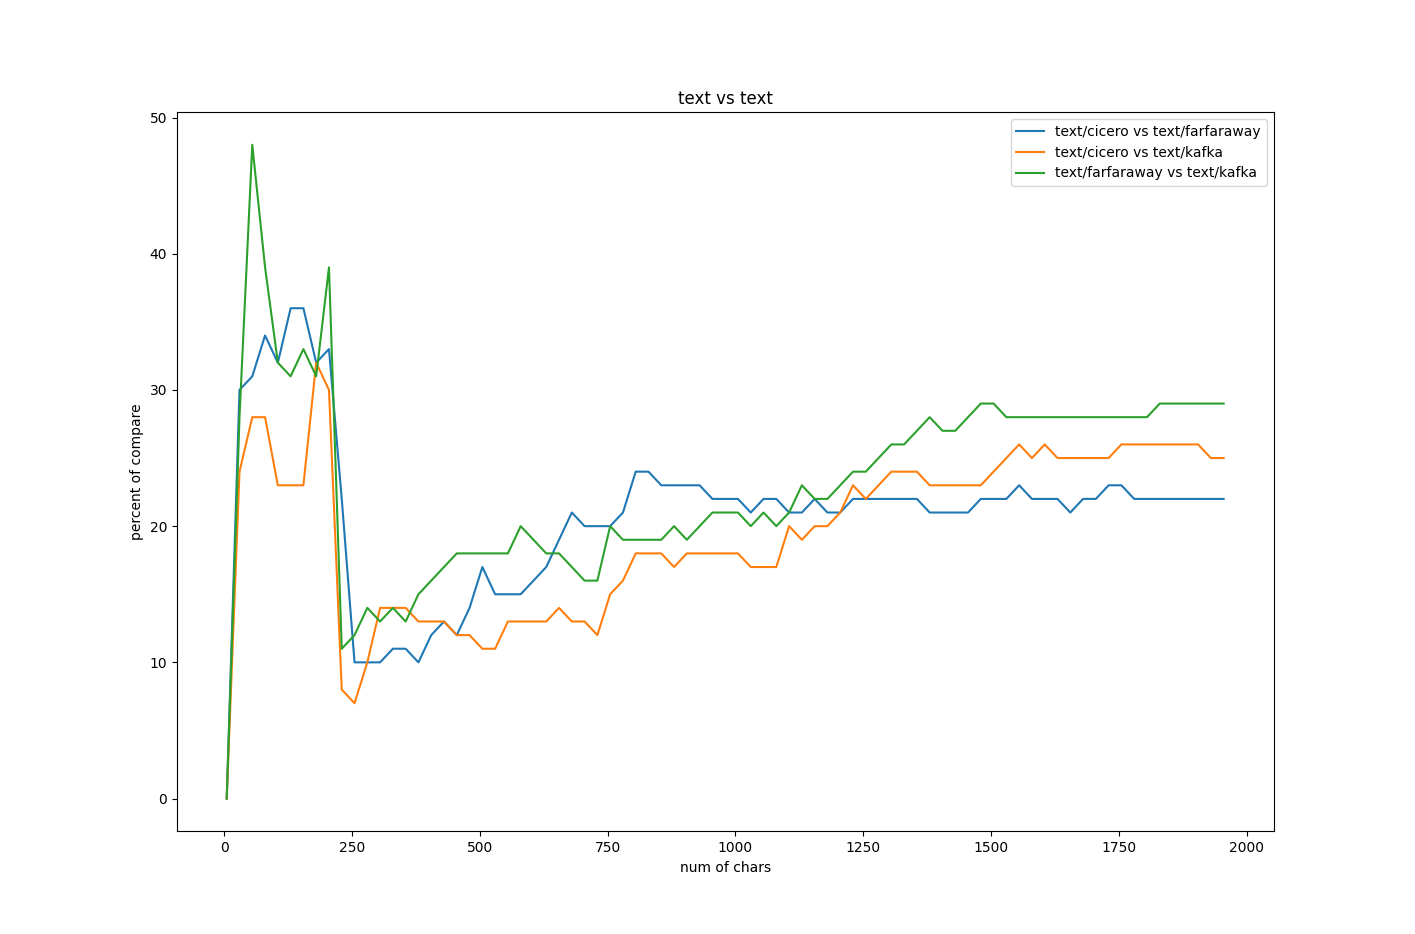
\includegraphics[scale=0.5]{pic/1.png}

Отметка совпадений держится на уровне 30 процентов и ниже, конечно, ведь тексты проверяются абсолютно разные, маловероятно, что авторы копировали работы друг у друга, так еще и 2 тысячи символов немного маленькая цифра, да и текстов мало, всего 3.

\section{Текст vs random letters}
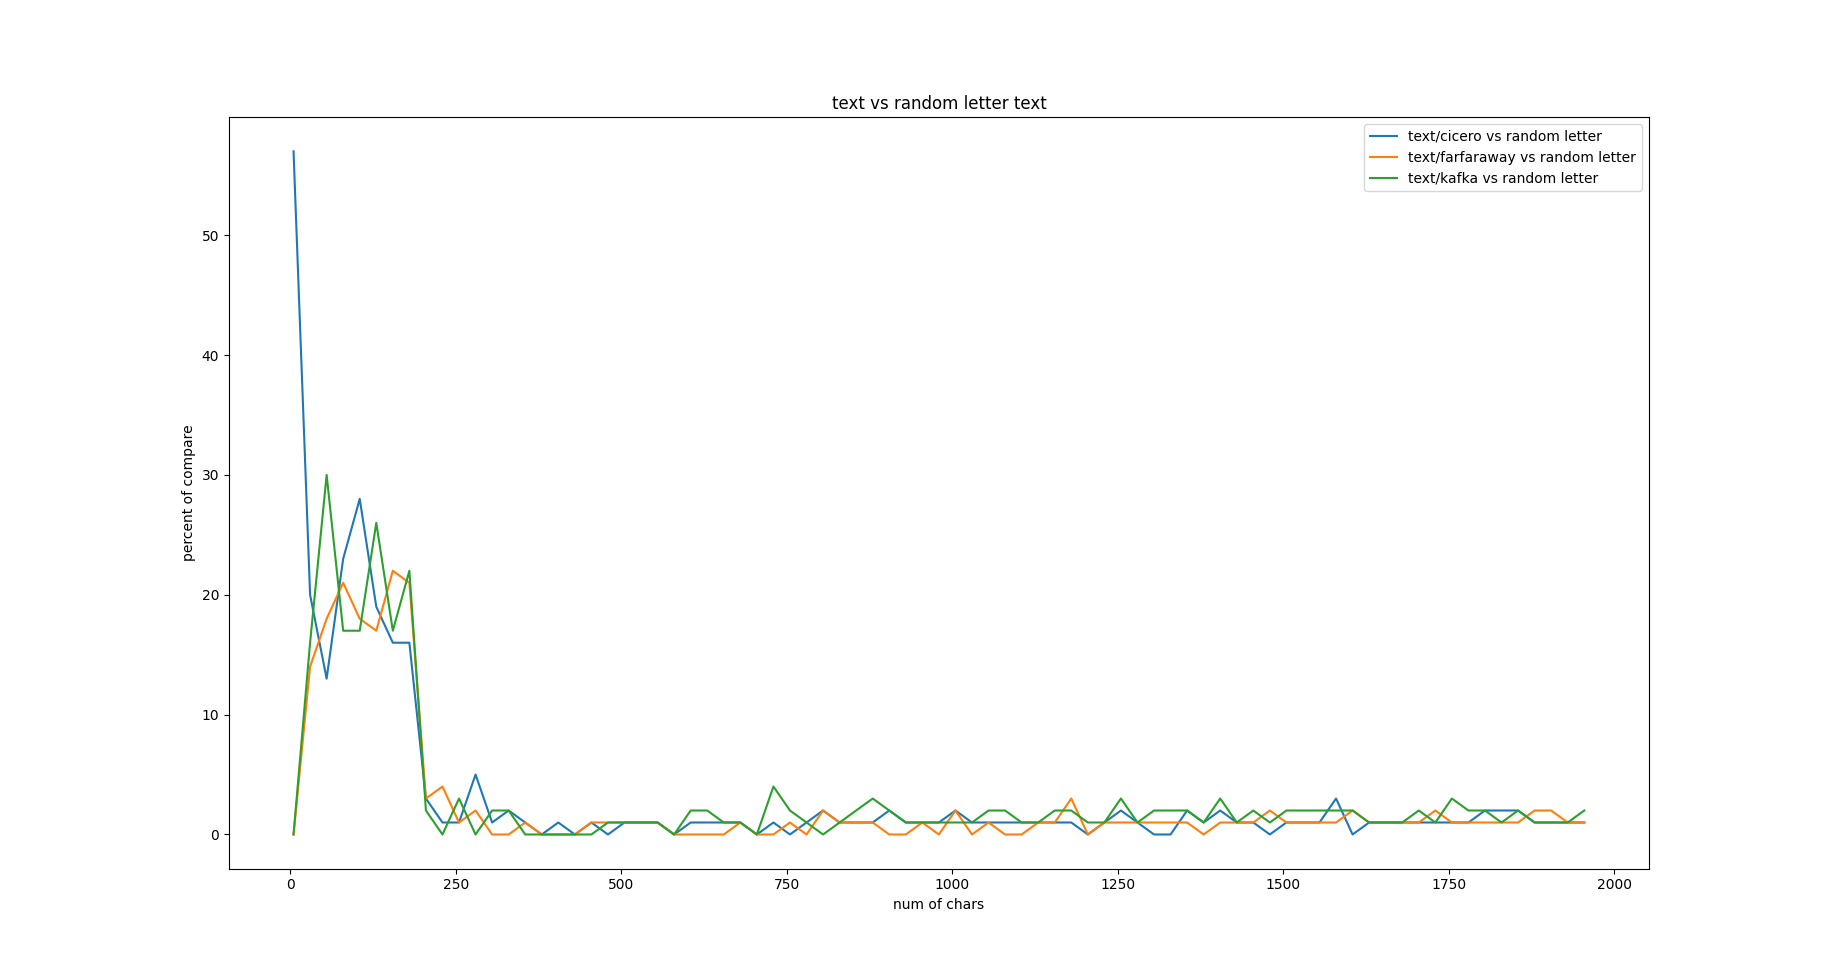
\includegraphics[scale=0.4]{pic/2.png}

Полный провал, как ни разбивай на рандомные слова, слова сделаны из каши, логической оценке не подлежат и вообще не похожы на что либо. Отсюда и такой маленький процент на больших текстах. Удивительно, что на маленькой длине процент держится около 30, может какие то слова образовались, оказавшись шумом в функции сравнения.

\section{Текст vs random words}
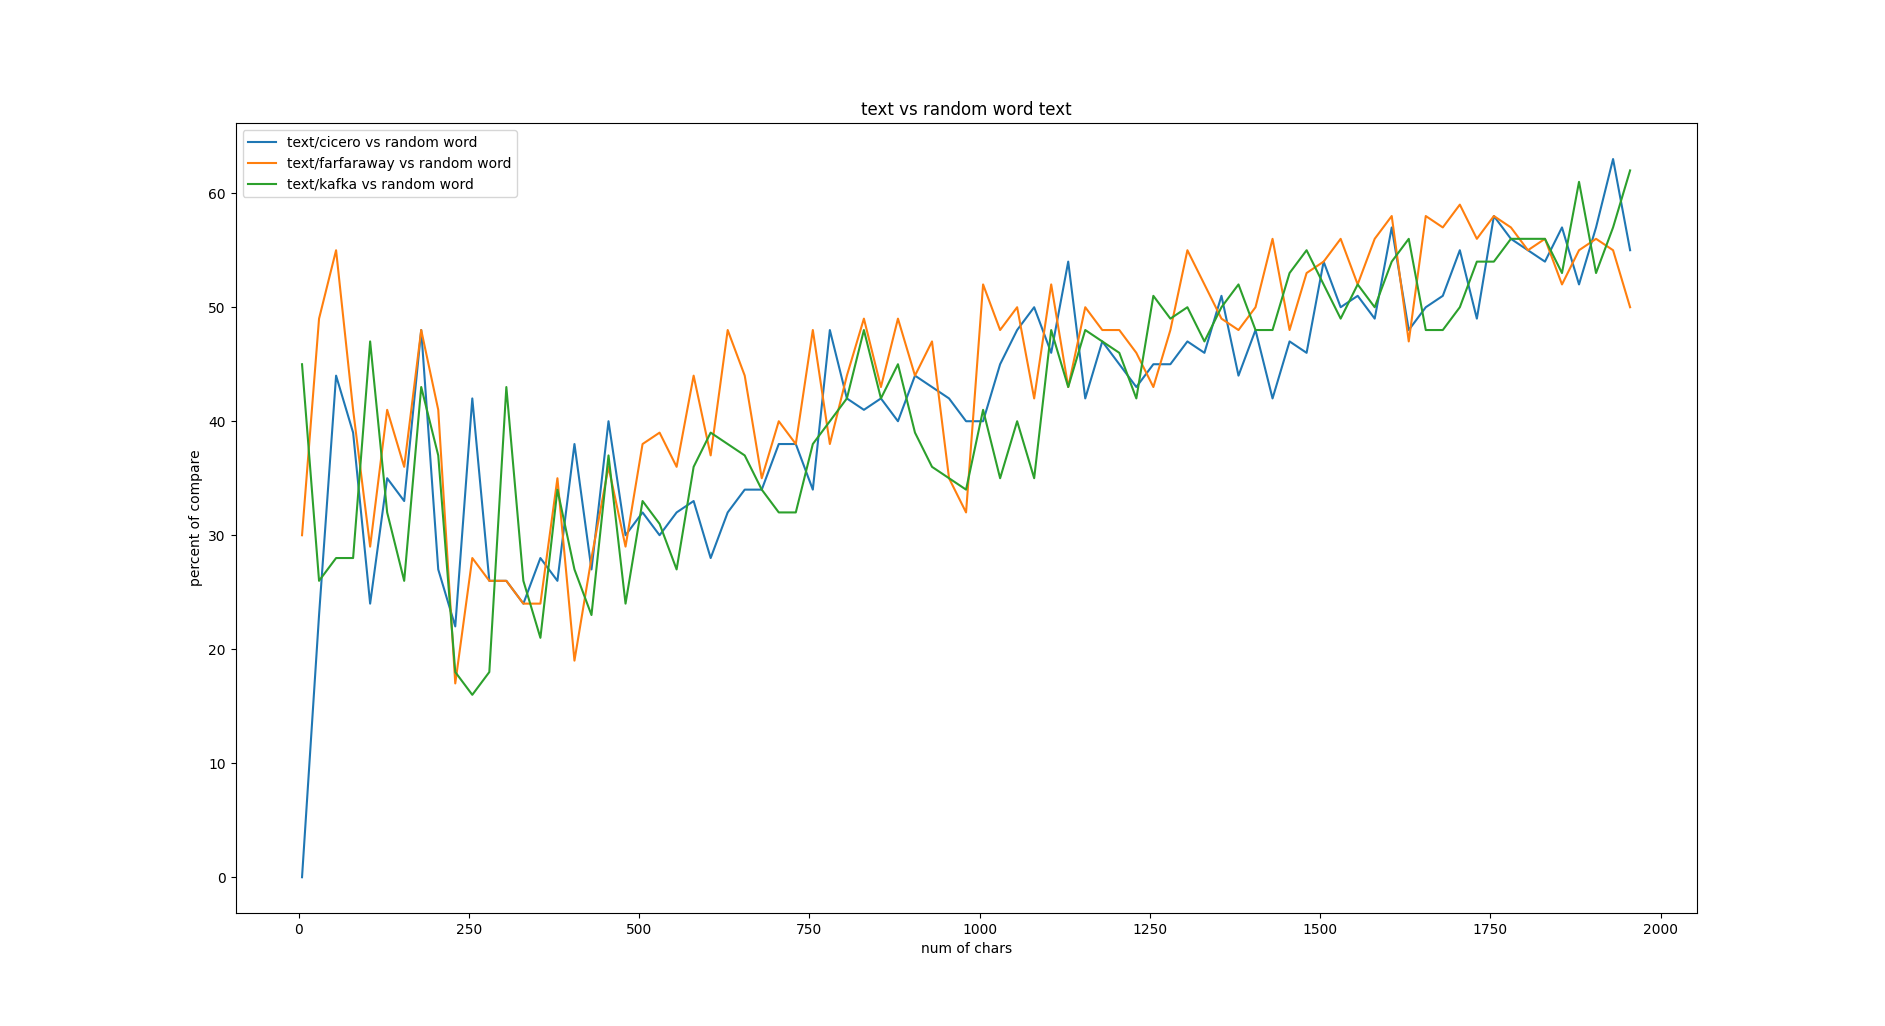
\includegraphics[scale=0.4]{pic/3.png}

Стоит сказать, что эти random words были взяты из совокупности текстов, в данном случае всех трех, уровень в 60 процентов можно обьяснить очень просто: 30 процентов взялись из обычно сравнения показанного в 1 тесте, а еще 30 взялись из за того, что текст был составлен почти на треть из сравниваемого текста. Стоит конечно для наглядности и проверки гипотезы набрать слов только из других текстов, но я более чем уверен, уровень будет такой же как в 1 тесте, то есть около 30 процентов.


\section{random letters vs random letters}

\includegraphics[scale=0.4]{pic/4.png}

Очередной полый провал, рандомные буквы собираются в псевдо слова, что то и совпадает, но не более чем шум. Для наглядности взял длину в 10 тысяч символов, забавно было узнать что отметка в 5 процентов держится и там, возможно функции распределния выбора случайных букв начинают повторяться, хотя врятли.


\section{random words vs random letters words}

\includegraphics[scale=0.4]{pic/5.png}

5 тестов из слов на основании всех трех текстов, боюсь представить какая там каша, на таких примерах статистическое сравнение работает хуже всего, никакой смысловой нагрузки текст не несет, что там что там, одинаково бессмысленный, что дает им полное право быть похожими, конечно склоняюсь к тому что на такой длине выборка начинает повторяться, проверить бы на текстах длинной от 15 до 30 тысяч символов.

\section{Информация о машине}

macOS Catalina 10.15.7

MacBook Pro (13-inch, 2017, Two Thunderbolt 3 ports)

Процессор 2,3 GHz 2‑ядерный процессор Intel Core i5

Память 8 ГБ 2133 MHz LPDDR3

Графика Intel Iris Plus Graphics 640 1536 МБ

\section{Заключение}

Помимо статистического сравнения, который является относительно быстрым, необходимо применять комбинированные алгоритмы с лексическим анализом, они дают ощутимый прирост точности неточного сравнения текстов. Только вопрос, где он более уместен, на больших текстах его особо не применить, скорость оченб маленькая. Чистый питонный fuzzywuzzy на тексте до 10 тысяч слов работал за 10-20 секунд, что уже долго.


% \pagebreak







